\begin{tikzpicture}[trim axis left]
\begin{axis}[
    % width of chart
    width=\textwidth,
    height=0.4\textheight,
    % no box, below chart, horizontal
    legend style={%
      draw=none,
      at={(0.5,-0.15)},
      anchor=north,
      legend columns=4,
      column sep = 1em,
      cells={align=center},
    },
    % log ticks with fixed point,
    % yticklabel={\pgfmathparse{pow(10,\tick-3)}\pgfmathprintnumber[fixed]{\pgfmathresult}}\,ms, % N ms along y-axis
    % xticklabel={\pgfmathparse{pow(5,\tick)}\pgfmathprintnumber[fixed]{\pgfmathresult}},
    xlabel near ticks,
    xlabel={Matrix size $n$ (for a Kalman filter, with $k=3n/5$)},
    ylabel near ticks,
    ylabel={Execution time of one call to Kalman filter ($\mu$s)},
    xmode = log,
    log basis x = {5},
    axis line style={opacity=0}, % hide y axis
    major tick style={draw=none}, % no ticks
    ymode=log, % log scale for y
    log basis y = {10}, % log base 10
    ymajorgrids, % rows of lines
    major grid style={gray, line width=1pt},
]

  % CBLAS
    \addplot+ [
        violet,
        mark options={fill=violet},
        error bars/.cd, y dir=both, y explicit,
    ] table [
        y error plus=ey+,
        y error minus=ey-,
    ] {
         x         y     ey+     ey-
         5        24       0       0
        25       104       1       1
       125      1803      64      57
       625    187667   36281   36281
      3125  15651064  530675  530675
  };

  % LT4LA
    \addplot+ [
        ForestGreen,
        mark options={fill=ForestGreen},
        error bars/.cd, y dir=both, y explicit,
    ] table [
        y error plus=ey+,
        y error minus=ey-,
    ] {
         x         y     ey+     ey-
         5        41       1       1
        25       133       2       2
       125      1678      36      33
       625    180575   38386   38386
      3125  16061291  193746  193746
  };

  \legend{CBLAS,LT4LA}

\end{axis}
\end{tikzpicture}
